\section{Virtualization Technologies}
\label{sec:leavingvirtualization}

A broad, loose, and multiple-purpose oriented definition of (computer) virtualization can be taken out of the excellent essay that is~\cite{introvirtualization}:
\begin{displayquote}
Virtualization is a framework or methodology of dividing the resources of a computer into multiple execution environments, by applying one or more concepts or technologies such as hardware and software partitioning, time-sharing, partial or complete machine simulation, emulation, quality of service, and many others.
\end{displayquote}

However, to narrow down the definition in this case, we can say that a virtual machine, under  a modern multiprocess OS, is a software-based execution \emph{context} where one or more programs can be run in isolation when observed outside of that context.
The degree by which this isolation is provided varies on different kinds of virtualization.

In full-system virtualization (also called hardware-level virtualization), the aforementioned OS is a specialized one, called hypervisor or \gls{vmm}.
The \gls{vmm} emulates a fully-fledged computer, the \gls{vm}, with CPUs, RAM, peripheral devices (e.g. \glspl{nic}, disks), etc.; therefore the \gls{vm}, indistinguishable from a real machine, can run a standard OS, which is then called the guest OS.
Usually, the term \gls{vm}, without any more information, refers to a full-system virtual machine.

Hypervisors such as, for example, VMware Workstation\footnote{\url{https://www.vmware.com/products/workstation-pro.html}} (and free alternatives, like VirtualBox\footnote{\url{https://www.virtualbox.org}} from Sun, now Oracle) that run along a standard OS such as Windows, macOS, or Linux in the same host and rely on the OS for some operations are called type-II or hosted hypervisors.
Others, such as VMware ESXi, Citrix Xen, Microsoft Hyper-V, Apple's Hypervisor, or KVM (the last three are provided by Windows, macOS, and Linux, respectively~\cite{whatiskvm,applehypervisor,hyperv}) that run stand-alone (ESXi) or rely on the standard OS only for resource management (all other examples), are called type-I, bare metal, or native hypervisors.

In OS-based virtualization, the OS creates separated contexts, called containers, that share the base OS kernel, but run in isolation with regard to other containers.
They are, when compared with \glspl{vm}, less resource hungry, and as such are also designated as a lightweight virtualization technology.

Linux has included in-kernel support for containerization for many years, but there was a recent upsurge in the use of containers as a result of Docker Inc.'s work on a string of technologies that very much simplify the use of containers~\cite{hwswvirt,virtessentials}.
The a schematic depiction of the difference between full-system virtualization and containers is offered in~\ref{fig:docker-vs-vms}, taken from~\cite{dockercontreplacingvms}.

% As~\cite{introvirtualization} describes, full virtual machines was typically a costly thing to do, especially on x86-based machines.
% However, the article is question is quite old.
% Even though there are more lightweight alternatives, presented afterwards, full-blown virtual machines are nowadays lighter, modern x86 processors provide hardware acceleration techniques to make it closer to native as well, and the sheer capacity of commodity hardware is also bigger than ever~\cite{virtualizationcontainerization}.

% However, other solutions exist that provide lower isolation levels (from an implementation standpoint) that can suffice for certain applications, as shown in later chapters. Nowadays, this concept is usually called containers.
% A container is a process running on the host's OS which resorts to technologies like \emph{Cgroups} and \emph{namespaces}, both provided by the Linux kernel, to be able to isolate its child processes from the host's or other containers' processes, namely in aspects of networking.
% However, the kernel is actually the same, which reduces the overhead dramatically~\cite{comparativevmscontainers}.

% A particular container infrastructure, very popular nowadays is Docker, which uses the aforementioned Linux kernel technologies but provides a whole set of tools that make working with containers, pre-defining \emph{images} to run on containerized infrastructure and distributing them, configuring, and even transparently providing a thin Linux virtual machine for non-Linux desktop environments.

% A high-level illustration of the difference between applications running on ``regular,'' full-blown VMs and applications running over Docker (here, Docker represents the full set of OS-functionality and APIs it abstracts to provide a ``container infrastructure'') is offered by figure~\ref{fig:docker-vs-vms}, taken from~\cite{dockercontreplacingvms}.

% Figure fig:docker-vs-vms
\begin{figure}
  \centering
  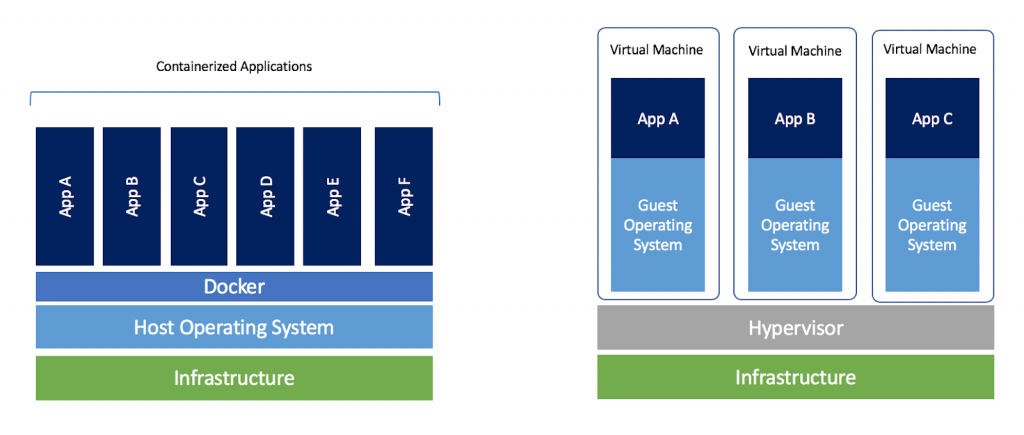
\includegraphics[width=0.8\textwidth]{docker-vs-vms}
  \caption{\textquote{Containers versus Virtual Machines}}
  \label{fig:docker-vs-vms}
\end{figure}


% end of section leavingvirtualizationtechnologies
